\documentclass[12pt,letter]{article}
\usepackage[moduleName={Super ADSR}]{KautenjaDSP}
\begin{document}
\titlePage{img/Logo}{img/Module}{img/KautenjaDSP}

% -------------------
% MARK: Overview
% -------------------

\section{Overview}

Super ADSR is a Eurorack module that emulates the ADSR envelope generator from the S-SMP sound chip on the Super Nintendo Entertainment System (SNES). The ADSR on the SNES has (1) a linear attack stage, followed by (2) a non-linear decay stage that falls to a (3) sustain level that maintains for a (4) sustain rate or until key-off. On key-off the envelope quickly releases to zero in a way that produces minimal popping and clicks. Super ADSR provides the key features of the ADSR of the S-SMP chip, namely,
\begin{itemize}
  \item \textbf{Dual ADSR:} Two envelope generators!
  \item \textbf{Bipolar Level Control:} Control the total height of the envelope (i.e., the point the attack stage stops at), including the ability to polarize the envelope into negative voltages.
  \item \textbf{LED Indicators:} LEDs indicate the active stage and strength / polarity of the envelope output.
\end{itemize}

\begin{figure}[!b]
\centering
\includegraphics[width=0.5\textwidth]{img/Chip}
\caption{\small The S-SMP module from the SNES. The S-SMP included two discrete microprocessors: the SPC700, and the S-DSP. The SPC700 performed primary computation, while the S-DSP performed DSP specific computations, like BRR decoding, sample playback, applying the echo effect, mixing levels, etc. The SPC700 and S-DSP shared $64KB$ of total RAM that was used for BRR sample data and the echo buffer. The digital audio is decoded back to an analog signal by a 16-bit DAC and amplified using an Op-Amp. Before digital-to-analog conversion, the output audio is low-pass filtered by a Gaussian filter that gives the S-SMP chip a distinctive sound.}
\end{figure}

% -------------------
% MARK: Panel Layout
% -------------------

\clearpage
\section{Panel Layout}

\begin{figure}[!htp]
\centering
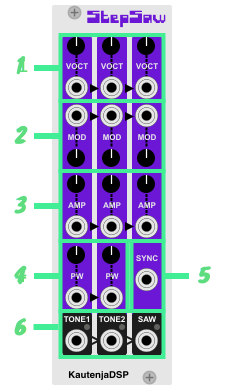
\includegraphics{img/Interface}
\end{figure}

\subsection{Envelope Generator Stages}

The envelope generator section provides control over the envelope generator parameters for each processing lane on the module.
% Figure~\ref{fig:envelope-generator} depicts the stages in the envelope generator, where
The envelope generator has five total parameters, namely,
\begin{itemize}
 \item \textbf{Total Level ($\pm$)} controls the polarity and highest amplitude of the envelope generator;
 \item \textbf{Attack (\texttt{A})} controls the amount of time spent in the attack stage from $0V$ to the highest voltage according to to the total level;
 \item \textbf{Decay Rate (\texttt{D})} controls the angle of amount of time in the decay stage from the highest amplitude to the sustain level;
 \item \textbf{Sustain Level (\texttt{S}):} controls the amplitude where sustained notes are held;
 \item \textbf{Release Rate (\texttt{RR})} controls the amount of decay from the sustain level. This will continue indefinitely unless \texttt{key off} occurs.
\end{itemize}

When a \texttt{key off} event occurs, the envelope generator enters a very short release stage that prevents clicks and pops. This is a feature of the original S-SMP chip, and has no controls.

\subsection{Ports}

The envelope generator functions using only gate signals, and cannot be triggered. The \textbf{GATE} input accepts a gate signal that goes high at $2V$ and triggers the envelope generators attack stage. The \textbf{RETRIG} input goes high at $2V$ and can be used to re-trigger the attack stage of the envelope generator without needing to release the gate signal. The output of the envelope generator is available on two separate ports the \textbf{OUT} port produces the standard output, while the \textbf{INV} port produces an inverted output that can be used for ducking, etc.

\end{document}
